\documentclass[11pt,utf8,notheorems,compress,t]{beamer}
\usepackage{etex}

\usepackage{pgfpages}
\setbeameroption{show notes on second screen}
\setbeamertemplate{note page}[plain]
\newcommand{\jnote}[2]{\only<#1>{\note{\setlength\parskip{\medskipamount}\footnotesize\justifying#2\par}}}

% Workaround for the issue described at
% https://tex.stackexchange.com/questions/164406/beamer-using-href-in-notes.
\newcommand{\fixedhref}[2]{\makebox[0pt][l]{\hspace*{\paperwidth}\href{#1}{#2}}\href{#1}{#2}}

\usepackage[english]{babel}

\usepackage{mathtools}
\usepackage{booktabs}
\usepackage{stmaryrd,wasysym}
\usepackage{array}
\usepackage{ragged2e}
\usepackage{multicol}
\usepackage{tabto}
\usepackage{xstring}
\usepackage{ifthen}
\usepackage{soul}\setul{0.3ex}{}
\usepackage[all]{xy}
\xyoption{rotate}
\usepackage{tikz}
\usetikzlibrary{calc,shapes,shapes.callouts,shapes.arrows,patterns,fit,backgrounds,decorations.pathmorphing}
\hypersetup{colorlinks=true}

\usepackage{pifont}
\newcommand{\cmark}{\ding{51}}
\newcommand{\xmark}{\ding{55}}
\DeclareSymbolFont{extraup}{U}{zavm}{m}{n}
\DeclareMathSymbol{\varheart}{\mathalpha}{extraup}{86}

\graphicspath{{images/}}

\usepackage[protrusion=true,expansion=true]{microtype}

\setlength\parskip{\medskipamount}
\setlength\parindent{0pt}

\title{How not to constructivize cohomology}
\author{Ingo Blechschmidt}
\date{October 6th, 2018}

\useinnertheme[shadow=true]{rounded}
\setbeamerfont{block title}{size={}}

\useinnertheme{rectangles}

\usecolortheme{orchid}
\usecolortheme{seahorse}
\definecolor{mypurple}{RGB}{150,0,255}
\setbeamercolor{structure}{fg=mypurple}
\definecolor{myred}{RGB}{150,0,0}
\setbeamercolor*{title}{bg=myred,fg=white}
\setbeamercolor*{titlelike}{bg=myred,fg=white}
\setbeamercolor{frame}{bg=black}

\usefonttheme{serif}
\usepackage[T1]{fontenc}
\usepackage{libertine}

\newcommand{\A}{\mathcal{A}}
\renewcommand{\AA}{\mathbb{A}}
\newcommand{\E}{\mathcal{E}}
\newcommand{\F}{\mathcal{F}}
\renewcommand{\G}{\mathcal{G}}
\newcommand{\GG}{\mathbb{G}}
\renewcommand{\O}{\mathcal{O}}
\newcommand{\K}{\mathcal{K}}
\newcommand{\NN}{\mathbb{N}}
\newcommand{\QQ}{\mathbb{Q}}
\newcommand{\RR}{\mathbb{R}}
\newcommand{\TT}{\mathbb{T}}
\newcommand{\PP}{\mathbb{P}}
\newcommand{\ZZ}{\mathbb{Z}}
\renewcommand{\P}{\mathcal{P}}
\newcommand{\ppp}{\mathfrak{p}}
\newcommand{\defeq}{\vcentcolon=}
\newcommand{\defeqv}{\vcentcolon\equiv}
\newcommand{\Sh}{\mathrm{Sh}}
\newcommand{\GL}{\mathrm{GL}}
\newcommand{\Zar}{\mathrm{Zar}}
\newcommand{\op}{\mathrm{op}}
\newcommand{\Set}{\mathrm{Set}}
\newcommand{\Eff}{\mathrm{Ef{}f}}
\newcommand{\Sch}{\mathrm{Sch}}
\newcommand{\Aff}{\mathrm{Aff}}
\newcommand{\LRS}{\mathrm{LRS}}
\newcommand{\Hom}{\mathrm{Hom}}
\newcommand{\Spec}{\mathrm{Spec}}
\newcommand{\lra}{\longrightarrow}
\newcommand{\RelSpec}{\operatorname{Spec}}
\renewcommand{\_}{\mathpunct{.}}
\newcommand{\?}{\,{:}\,}
\newcommand{\speak}[1]{\ulcorner\text{\textnormal{#1}}\urcorner}
\newcommand{\ull}[1]{\underline{#1}}
\newcommand{\affl}{\ensuremath{{\ull{\AA}^1}}}
\newcommand{\Ll}{\vcentcolon\!\Longleftrightarrow}
\newcommand{\inv}{inv.\@}
\newcommand{\seq}{\vdash_{\!\!\!\vec x}}

\setbeamertemplate{blocks}[rounded][shadow=false]

% Adapted from https://latex.org/forum/viewtopic.php?t=2251 (Stefan Kottwitz)
\newenvironment<>{hilblock}{
  \begin{center}
    \begin{minipage}{9.05cm}
      \setlength{\textwidth}{9.05cm}
      \begin{actionenv}#1
        \def\insertblocktitle{}
        \par
        \usebeamertemplate{block begin}}{
        \par
        \usebeamertemplate{block end}
      \end{actionenv}
    \end{minipage}
  \end{center}}

\newcommand{\bignumber}[1]{
  \renewcommand{\insertenumlabel}{#1}\scalebox{1.5}{\usebeamertemplate{enumerate item}}
}
\newcommand{\bigheart}{
\includegraphics{heart}}

\newenvironment{changemargin}[2]{%
  \begin{list}{}{%
    \setlength{\topsep}{0pt}%
    \setlength{\leftmargin}{#1}%
    \setlength{\rightmargin}{#2}%
    \setlength{\listparindent}{\parindent}%
    \setlength{\itemindent}{\parindent}%
    \setlength{\parsep}{\parskip}%
  }%
  \item[]}{\end{list}}

\tikzset{
  invisible/.style={opacity=0,text opacity=0},
  visible on/.style={alt={#1{}{invisible}}},
  alt/.code args={<#1>#2#3}{%
    \alt<#1>{\pgfkeysalso{#2}}{\pgfkeysalso{#3}}}
}

\newcommand{\pointthis}[3]{%
  \tikz[remember picture,baseline]{
    \node[anchor=base,inner sep=0,outer sep=0,color=blue!90] (#2) {#2};
    \node[visible on=#1,overlay,rectangle callout,rounded corners,callout
    relative pointer={(0.0cm,-0.5cm)},fill=blue!20] at ($(#2.north)+(-0.1cm,0.7cm)$) {#3};
  }%
}

\newcommand{\pointthisbelow}[3]{%
  \tikz[remember picture,baseline]{
    \node[anchor=base,inner sep=0,outer sep=0,color=blue!90] (#2) {#2};
    \node[visible on=#1,overlay,rectangle callout,rounded corners,callout
    relative pointer={(0.0cm,0.5cm)},fill=blue!20] at ($(#2.north)+(-0.1cm,-1.0cm)$) {#3};
  }%
}

% Adapted from https://latex.org/forum/viewtopic.php?t=2251 (Stefan Kottwitz)
\newenvironment<>{varblock}[2]{
  \begin{center}
    \begin{minipage}{#1}
      %\setlength{\textwidth}{#1}
      \begin{actionenv}#3
	\def\insertblocktitle{\centering #2}
	\par
	\usebeamertemplate{block begin}}{
        \par
        \usebeamertemplate{block end}
      \end{actionenv}
    \end{minipage}
  \end{center}
}

\setbeamertemplate{headline}{%
  \begin{beamercolorbox}[wd=\paperwidth,ht=2.25ex]{}%
    \insertsectionnavigationhorizontal{\paperwidth}{}{}%
  \end{beamercolorbox}%
  \vskip0pt%
}

\setbeamertemplate{frametitle}{%
  \vskip1.0em%
  \leavevmode%
  \begin{beamercolorbox}[dp=1ex,center]{}%
      \usebeamercolor[fg]{item}{\textbf{{\Large \insertframetitle}}}
  \end{beamercolorbox}%
}

\setbeamertemplate{navigation symbols}{}

\newcounter{framenumberpreappendix}
\newcommand{\backupstart}{
  \setcounter{framenumberpreappendix}{\value{framenumber}}
}
\newcommand{\backupend}{
  \addtocounter{framenumberpreappendix}{-\value{framenumber}}
  \addtocounter{framenumber}{\value{framenumberpreappendix}}
}

\newcommand{\insertframeextra}{}
\setbeamertemplate{footline}{%
  \begin{beamercolorbox}[wd=\paperwidth,ht=2.25ex,dp=1ex,right,rightskip=1mm,leftskip=1mm]{}%
    % \inserttitle
    \hfill
    \insertframenumber\insertframeextra\,/\,\inserttotalframenumber
  \end{beamercolorbox}%
  \vskip0pt%
}

\newcommand{\hil}[1]{{\usebeamercolor[fg]{item}{\textbf{#1}}}}
\newcommand{\bad}[1]{\textcolor{red!90}{#1}}

\begin{document}

\addtocounter{framenumber}{-1}

{\usebackgroundtemplate{\begin{minipage}{\paperwidth}\vspace*{4.95cm}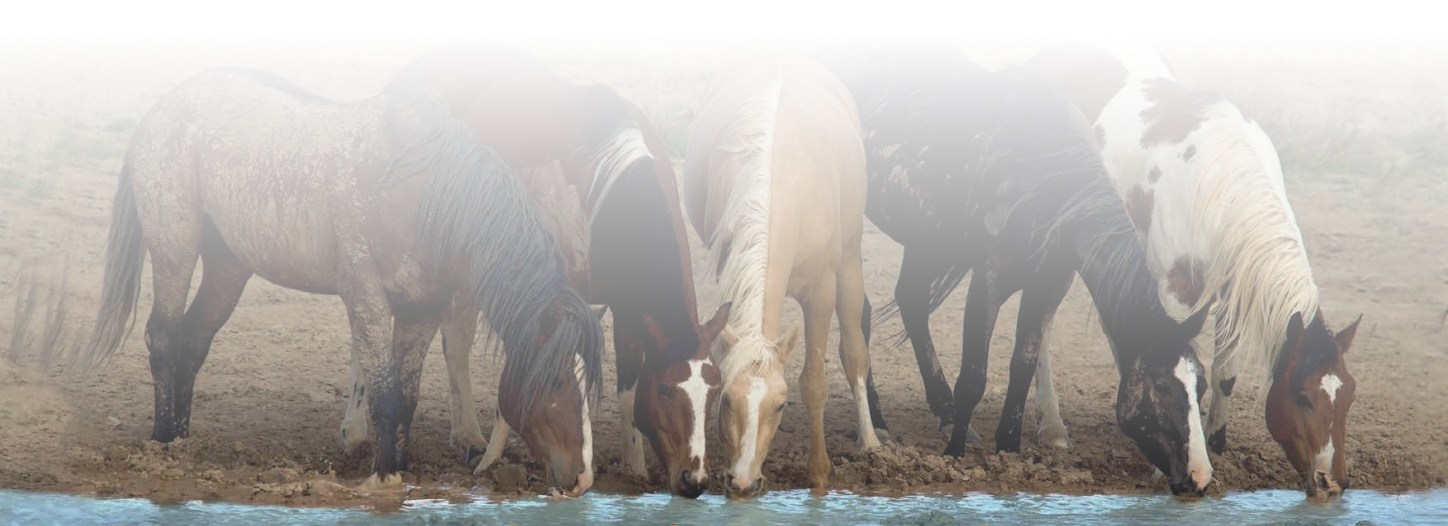
\includegraphics[width=\paperwidth]{topos-horses}\end{minipage}}
\begin{frame}[c]
  \centering

  \bigskip
  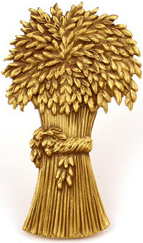
\includegraphics[width=0.2\textwidth]{sheaf}
  \bigskip

  \hil{How not to constructivize cohomology}

  \scriptsize
  \textit{-- interruptions welcome at any point --}
  \bigskip

  Ingo Blechschmidt \\
  University of Verona
  \bigskip

  104th Peripatetic Seminar on Sheaves and Logic in Amsterdam \\
  October 6th, 2018
  \par
\end{frame}}

\begin{frame}{Flabby sets}
  Let~$M$ be a set. A subset~$K \subseteq M$ is \ldots
  \begin{itemize}
    \item a \hil{subterminal} iff $\forall x,y \in K\_ x = y$.
    \item \mbox{a \hil{subsingleton} iff $\exists a \in M\_ \forall x \in K\_ x = a$, that is,} \\
    \mbox{\phantom{a \hil{subsingleton}} iff $K \subseteq \{ a \}$ for some~$a \in M$.}
  \end{itemize}

  Trivially, any subsingleton is a subterminal.

  \mbox{\textbf{Definition.}\visible<2->{\hil{$^\star$}}
  A set~$M$ is \hil{flabby} iff any subterminal is a subsingleton.}

  Any flabby set is inhabited.
  %Conversely, any inhabited set is flabby iff the law of excluded middle holds.

  \visible<4->{
    \textbf{Proposition.} Any set embeds into a flabby set.

    \justifying
    \textbf{Proof.} We have~$M \hookrightarrow P(M)$, and~$P(M)$ is flabby:
    Let~$K \subseteq P(M)$ be a subterminal. Then~$K \subseteq \{ \bigcup K \}$,
    for if~$A \in K$, then~$K = \{ A \}$ and hence~$A \in \{ \bigcup K \} = \{ A \}$.
  }

  \visible<5->{
    \bad{\textbf{Open question.}} Does any module embed into a flabby module?
  }

  \vfill
  \visible<3->{
    \small
    \hil{$^\star$ This talk is set in the context of constructive mathematics:} \\
    \hil{\phantom{$^\star$}} mathematics without $\varphi \vee \neg\varphi$,\ \ $\neg\neg\varphi \Rightarrow \varphi$,\ \ axiom of choice
  }

  \jnote{1-}{Any flabby set is inhabited, for there is always the empty
  subterminal.

  Conversely, given a set~$M$ inhabited by some element~$x_0 \in M$, it
  might appear that we have an easy proof that~$M$ is flabby: Any
  subterminal~$K \subseteq M$ is empty or of the form~$K = \{ x \}$ for some~$x
  \in M$. In the first case, $K$ is a subsingleton for~$K \subseteq \{x_0\}$,
  and in the second case,~$K$ is a subsingleton for~$K \subseteq \{x\}$.

  Hence it might appear that the definition doesn't make much sense, since it
  might appear that flabbiness is equivalent to being inhabited.}

  \jnote{2-}{However, one always has to look out for the fine print.}

  \jnote{3-}{In constructive mathematics, the condition for a set to be flabby
  is nontrivial. We'll see later that the condition is also interesting for
  classical mathematics, if interpreted internally to suitable toposes.}

  \jnote{4-}{Even though constructively we can't show that any inhabited set is
  flabby, we can still verify that there are \emph{enough flabby sets}.}
  \jnote{5-}{However it's unknown whether there are \emph{enough flabby
  modules}. (A module is \emph{flabby} if and only if its underlying set is.)
  We'll see what the significance of this open question is later on.}
\end{frame}


\section[Cohomology]{Sheaf cohomology}

\newcommand{\smallsphere}{\ensuremath{\vcenter{\hbox{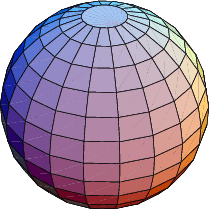
\includegraphics[height=1em]{sphere}}}}}
\newcommand{\smalltorus}{\ensuremath{\vcenter{\hbox{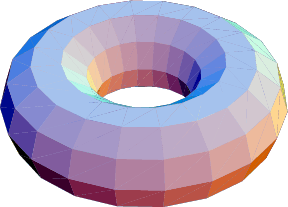
\includegraphics[height=1em]{torus}}}}}

{\usebackgroundtemplate{\begin{minipage}{\paperwidth}\vspace{5.6cm}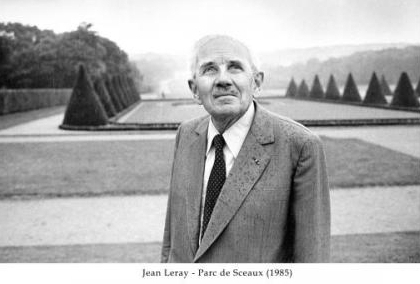
\includegraphics[width=\paperwidth]{leray}\end{minipage}}
\begin{frame}{Singular cohomology}
  \centering

  Is $\vcenter{\hbox{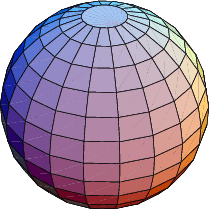
\includegraphics[height=0.1\textwidth]{sphere}}}$ homeomorphic to
  $\vcenter{\hbox{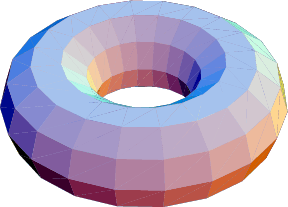
\includegraphics[height=0.1\textwidth]{torus}}}$? No:
  \begin{align*}
    H^0_{\text{sing}}(\smallsphere,\ZZ) &\cong \ZZ &
    H^1_{\text{sing}}(\smallsphere,\ZZ) &\cong 0 &
    H^2_{\text{sing}}(\smallsphere,\ZZ) &\cong \ZZ \\
    H^0_{\text{sing}}(\smalltorus,\ZZ) & \cong \ZZ &
    H^1_{\text{sing}}(\smalltorus,\ZZ) & \cong \ZZ \oplus \ZZ &
    H^2_{\text{sing}}(\smalltorus,\ZZ) & \cong \ZZ
  \end{align*}

  \begin{block}{}
    \justifying
    Given~$f : X \to B$, can we compute the cohomology of~$X$ if we
    understand the cohomology of~$B$ and the cohomology of the fibers of~$f$?
  \end{block}{}

  \jnote{1-}{Associated to any topological space~$X$ and any abelian group~$A$
  are the groups~$H^n_{\text{sing}}(X, A)$, the singular cohomology groups
  of~$X$ with coefficients in~$A$. They depend functorially on~$X$; hence one
  of many of their applications is to verify that given spaces are not
  homeomorphic.

  Given a space~$X$, we can hope that we can write~$X$ as the
  codomain of a continuous map~$f : X \to B$, in such a way that the base space~$B$
  and the fibers of~$f$ are in some sense easy to understand. In such a situation we
  could ask whether the cohomology of~$X$ can be computed from the cohomology
  of~$B$ and the cohomology of the fibers.

  The answer, given by Jean Leray in the 1940s, is: Yes, we can, but the
  framework of singular cohomology is too rigid for this task. For a positive answer we have
  to generalize to sheaf cohomology. And thus, the notion of sheaves was born.}
\end{frame}}

\begin{frame}{Sheaf cohomology}
  \vspace*{-1.2em}
  \begin{varblock}{\textwidth}{}
    \justifying
    Let~$E$ be a sheaf of modules over a space~$X$.
    Let~$\Gamma$ be the global sections functor.
    Choose an \bad{injective resolution} $0 \to E \to I^0 \to I^1 \to \cdots$.
    Then the \hil{$\boldsymbol{n}$-th cohomology of $\boldsymbol{E}$ is}
    \begin{align*}
      H^n(X, E) &\defeq \text{$n$-th cohomology of $(0 \to \Gamma I^0 \to \Gamma I^1 \to \cdots)$} \\
      &\phantom{\vcentcolon}= \operatorname{ker}(\Gamma I^n \to \Gamma I^{n+1})\mathop{/}\operatorname{im}(\Gamma I^{n-1} \to \Gamma I^n).
    \end{align*}
  \end{varblock}

  \begin{itemize}
    \item The modules~$H^n(X, E)$ are important invariants.

          [ $\chi(X, \O_X) = 1 - \operatorname{genus}_X$,
          $(C \cdot C') = \chi(\O_C \otimes_{\O_X}^{\mathbb{L}} \O_C')$, \ldots ]
          \\[0.6em]
    \item Let~$A$ be an abelian group. Let~$X$ be semi-locally contractible.
          Then $H^n(X, \underline{A}) = H_{\text{sing}}^n(X, A)$
          \href{https://arxiv.org/abs/1602.06674}{[Sella 2016]}.
          \\[0.6em]
    \item Let~$f : X \to B$ be continuous. Then there is a spectral sequence
          $H^i(B, R^jf_*(E)) \Longrightarrow H^{i+j}(X, E)$.
  \end{itemize}

  \jnote{1-}{An injective resolution is a sequence of sheaves of modules and
  linear morphisms as indicated such that the sequence is \emph{exact}
  (the kernel of any outgoing morphism equals the image of the respective incoming
  morphism) and such that the sheaves~$I^n$ are injective (a notion recalled
  below).

  The fundamental fact of homological algebra is: Even though the sequence~$0
  \to I^0 \to I^1 \to \cdots$ can only fail to be exact at the front, the
  sequence~$0 \to \Gamma I^0 \to \Gamma I^1 \to \cdots$ of global sections can
  fail to be exact at any place. Sheaf cohomology measures the extent of this
  failure.

  The standard proof of the existence of injective resolutions requires Zorn's
  lemma and the law of excluded middle. Injective resolutions are not unique,
  but the resulting sheaf cohomology modules are unique up to isomorphism.
  A primer on these matters is located
  \fixedhref{https://rawgit.com/iblech/talk-homological-algebra/master/notes-derived-functors.pdf}{here}.

  The positive answer to the question posed on the previous slide is given by
  the spectral sequence displayed at the bottom of this slide. The sheaves~$R^n
  f_*(E)$ are called the \emph{higher direct images of~$E$} (along~$f$). Even
  if~$E$ is a constant sheaf, its higher direct images might not be. This is
  the reason why singular cohomology is too restrictive.

  The higher direct images~$R^n f_*(E)$ are defined exactly as the sheaf
  cohomology~$H^n(X, E)$, only with the global sections functor~$\Gamma$
  replaced by the pushforward functor~$f_*$. They are dubbed ``relative
  cohomology'', for instance because under some conditions, there are
  isomorphisms~$(R^n f_*(E))_b \cong H^n(X_b, E|_{X_b})$ where~$X_b$ is the
  fiber of~$b$ under~$f$. This talk presents a rigorous and general way to
  regard higher direct images as sheaf cohomology.}
\end{frame}


\section[Constructivism]{Constructive mathematics}

\begin{frame}{Constructive mathematics}
  \centering

  \vspace*{-1em}
  mathematics without $\varphi \vee \neg\varphi$,\ \ $\neg\neg\varphi \Rightarrow \varphi$,\ \ axiom of choice
  \bigskip

  \centering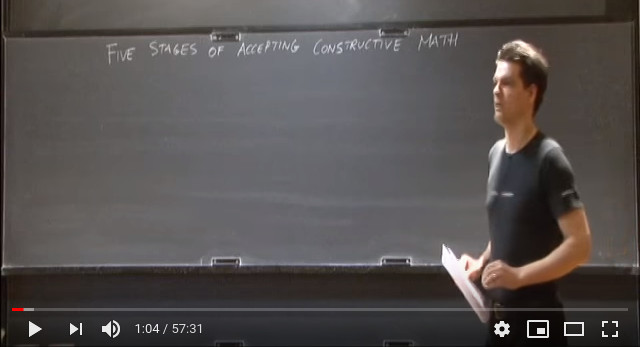
\includegraphics[width=0.5\textwidth]{andrej-bauer-five-stages} \\
  \scriptsize\href{https://video.ias.edu/members/1213/0318-AndrejBauer}{Andrej Bauer at an IAS talk}\par
  \small
  \bigskip

  \begin{columns}
    \begin{column}{0.50\textwidth}
      \centering
      \hil{Axiomatic freedom}

      \footnotesize
      \mbox{``Every map~$\NN \to \NN$ is computable.''}
      \mbox{``Every map~$\RR \to \RR$ is continuous.''}
      \mbox{``Every map~$\affl \to \affl$ is polynomial.''}
      \href{https://www.staff.science.uu.nl/~ooste110/realizability/arithcatsubmit.pdf}{\mbox{``Heyting Arithmetic has exactly one model.''}}
      \href{http://www1.maths.leeds.ac.uk/~pmtng/Slides/gambino-lisbon-jan2018.pdf}{\mbox{``The subsets of~$\{\heartsuit\}$ form a proper class.''}}
      \href{https://rawgit.com/iblech/mathezirkel-kurs/master/superturingmaschinen/slides-warwick2017.pdf}{\mbox{``There is an injection~$\RR \to \NN$.''}} \\
      \rotatebox{90}{\dots}
    \end{column}

    \begin{column}{0.50\textwidth}
      \centering
      \hil{Applications}

      \footnotesize
      \mbox{program extraction} \\
      \href{http://math.andrej.com/2008/08/13/intuitionistic-mathematics-for-physics/}{\mbox{synthetic differential geometry}} \\
      \href{https://rawgit.com/iblech/internal-methods/master/notes.pdf}{\mbox{synthetic algebraic geometry}} \\
      \href{https://www.dpmms.cam.ac.uk/~martin/Research/Oldpapers/synthetic91.pdf}{\mbox{synthetic domain theory}} \\
      \href{https://rawgit.com/iblech/internal-methods/master/slides-bayreuth2018.pdf}{\mbox{new reduction techniques in algebra}} \\
      \href{https://rawgit.com/iblech/internal-methods/master/}{\mbox{Bohr topos for quantum mechanics}} \\
      \rotatebox{90}{\dots}
    \end{column}
  \end{columns}

  \jnote{1-}{Constructive mathematics can be studied for philosophical reasons
  or out of general mathematical curiosity. But restricting to constructive
  reasoning in our proofs also yields concrete gains for
  classical mathematics.

  One of these is \emph{program extraction}: From any constructive proof, we can
  mechanically extract a program witnessing the proven statement. A basic
  example is that any constructive proof of the infinitude of primes yields an
  algorithm for computing primes (together with a termination and correctness
  proof).

  Another is that, since constructive mathematics is consistent with a number
  of anti-classical dream axioms, constructive mathematics allows to develop
  \emph{synthetic accounts} of several subjects. For instance, in synthetic
  algebraic geometry, a scheme is just a set, a morphism of schemes is just
  a map of sets, and any map of the ground field into itself is polynomial.

  There are also \emph{reduction techniques} which propose interesting deals. For
  instance, there is a technique which allows us to pretend that a reduced ring
  is Noetherian and in fact a field -- if in return we switch from classical
  reasoning to constructive. This particular technique has been used to turn
  the slightly convoluted multi-page proof of Grothendieck's generic
  freeness lemma into a simple one-paragraph argument.

  An informative and entertaining primer on constructive mathematics can be
  found in the linked talk recording by Andrej Bauer or his
  \fixedhref{https://www.ams.org/journals/bull/2017-54-03/S0273-0979-2016-01556-4/S0273-0979-2016-01556-4.pdf}{written
  notes} on the subject. Don't worry, the standard proof that~$\sqrt{2}$ is not rational is
  perfectly fine in constructive mathematics.
  }
\end{frame}

% DURING THE TALK: Zitat vorlesen
% Thus, contrary to how it may appear on the surface, doing mathematics
% ``constructively'' does not usually involve giving up important theorems, but
% rather finding the best way to state the definitions so as to make the
% important theorems constructively provable. That is, we may freely use the [law of
% excluded middle] when first investigating a subject, but once that subject is
% better understood, we can hope to refine its definitions and proofs so as to
% avoid that axiom.


\section{Relativization by internalization}

\begin{frame}{Relativization by internalization}
  \vspace*{-0.5em}
  Let~$X$ be a space. The \hil{internal language} of the topos~$\Sh(X)$ allows us to reason
  about sheaves on~$X$ in \hil{naive element-based terms}.

  \only<1>{
    \vspace*{0.5em}
    \centering
    \rotatebox{90}{\tiny\scalebox{0.8}{Illustration: Carina Willbold}}\hspace{-0.05cm}%
    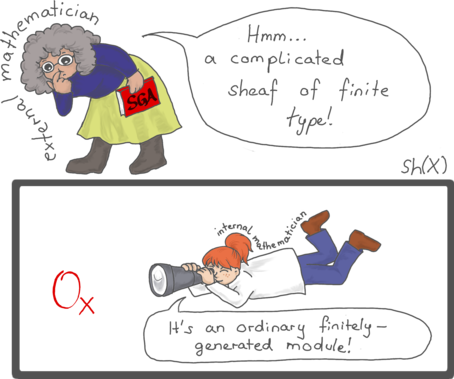
\includegraphics[width=0.7\textwidth]{external-internal-small}
    \par
  }
  \pause

  \begin{center}
    \small
    \begin{tabular}{ll}
      \toprule
      externally & internally to $\Sh(X)$ \\
      \midrule
      sheaf & set/type \\
      morphism of sheaves & map between sets \\
      %monomorphism of sheaves & injective map between sets \\
      %epimorphism of sheaves & surjective map between sets \\
      sheaf of cont.\@ real-valued functions & set of Dedekind reals \\
      %sheaf of modules & module \\
      %coherent sheaf of modules & coherent module \\
      over-locale~$f : Y \to X$ & locale~$I(Y)$ \\
      sheaf over~$Y$ & sheaf over~$I(Y)$ \\
      higher direct image $R^n f_* E$ & \bad{??} sheaf cohomology $H^n(I(Y), E)$ \\
      \midrule
      \pause
      \begin{minipage}{5.1cm}
        Every finite type sheaf of modules is finite locally free \emph{on a dense open}.
      \end{minipage} &
      \begin{minipage}{4.4cm}
        Every finitely generated vector space is \emph{not not} finite free.
      \end{minipage} \\
      \midrule
      \begin{minipage}{5.1cm}
        In continuous families of continuous functions with opposite signs,
        zeros can locally be picked continuously.
      \end{minipage} &
      \begin{minipage}{4.4cm}
        \raggedright
        The intermediate value theorem holds.
      \end{minipage} \\
      \midrule
      \begin{minipage}{5.1cm}
        \raggedright
        Grothendieck's generic freeness lemma holds.
      \end{minipage} &
      \begin{minipage}{4.2cm}
        \raggedright
        (Some trivial observation about modules over fields.)
      \end{minipage} \\
      \bottomrule
    \end{tabular}
  \end{center}

  \jnote{2-3}{The internal language of a topos~$\E$ is a device which defines
  for any formula~$\varphi$ of a certain language (a form of extensional type
  theory) what it means for~$\varphi$ to hold \emph{internally to~$\E$},
  written~``$\E \models \varphi$''. This translation process is sound with
  respect to intuitionistic logic; hence any theorem of constructive
  mathematics is valid in any topos. Only few toposes validate classical logic
  (for instance~$\Sh(X)$ does if~$X$ is a discrete space and the law of
  excluded middle is available in the metatheory).

  As a special case, the internal language of the topos~$\Set$ is just the
  usual mathematical language; more formally, $\Set \models \varphi$ if and
  only if~$\varphi$.}

  \jnote{3}{The intermediate value theorem (``any continuous function with
  opposite signs has a zero'') doesn't admit a constructive proof, because for
  most spaces~$X$ the external translation~$\Sh(X) \models \text{IVT}$ is not
  true -- it's not true that in continuous families of continuous functions
  with opposite signs, zeros can locally be picked continuously, as
  \fixedhref{https://raw.githubusercontent.com/iblech/internal-methods/master/images/zeros-in-families.mp4}{this
  video shows}.

  Over reduced schemes, every finite type sheaf of modules is finite locally free on a
  dense open. This statement (``important hard exercise'' 13.7.K in
  \fixedhref{http://math.stanford.edu/~vakil/216blog/FOAGnov1817public.pdf}{[Vakil
  2017]}) is just the external translation of the easy-to-prove internal
  statement that every finitely generated vector space does \emph{not not}
  admit a finite basis. (A scheme is reduced if and only if its structure sheaf
  looks like a field from the internal point of view (in the sense that $1 \neq
  0$ and~$\neg(\text{$x$ invertible}) \Rightarrow x = 0$). This is why the
  reducedness condition is important.)}

  \jnote{4-}{Excellent references on the internal language include:
  \begin{center}
    \fixedhref{https://www.oliviacaramello.com/Papers/Papers.htm}{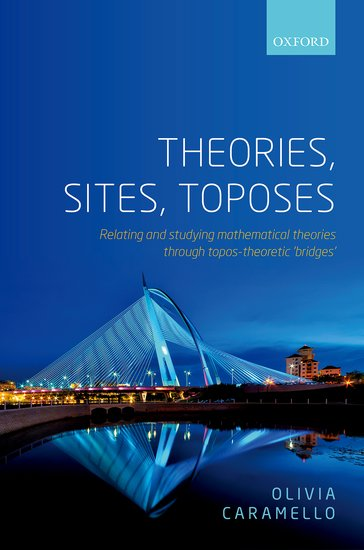
\includegraphics[height=3.5cm]{olivia-tst}}
    \fixedhref{https://store.doverpublications.com/0486450260.html}{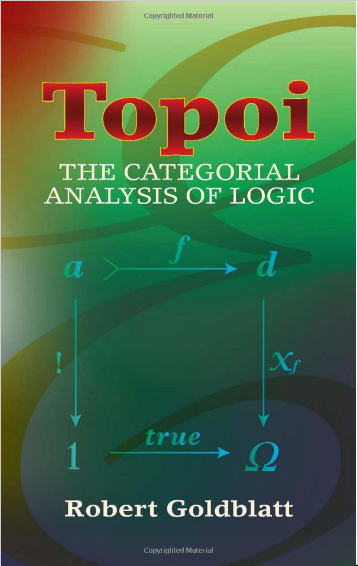
\includegraphics[height=3.5cm]{goldblatt-logic}}
    \fixedhref{https://www.worldcat.org/title/sheaves-in-geometry-and-logic-a-first-introduction-to-topos-theory/oclc/24428855}{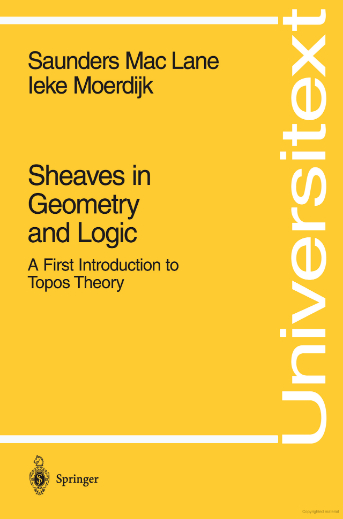
\includegraphics[height=3.5cm]{moerdijk-mac-lane-sheaves}}
    \fixedhref{https://www2.mathematik.tu-darmstadt.de/~streicher/CTCL.pdf}{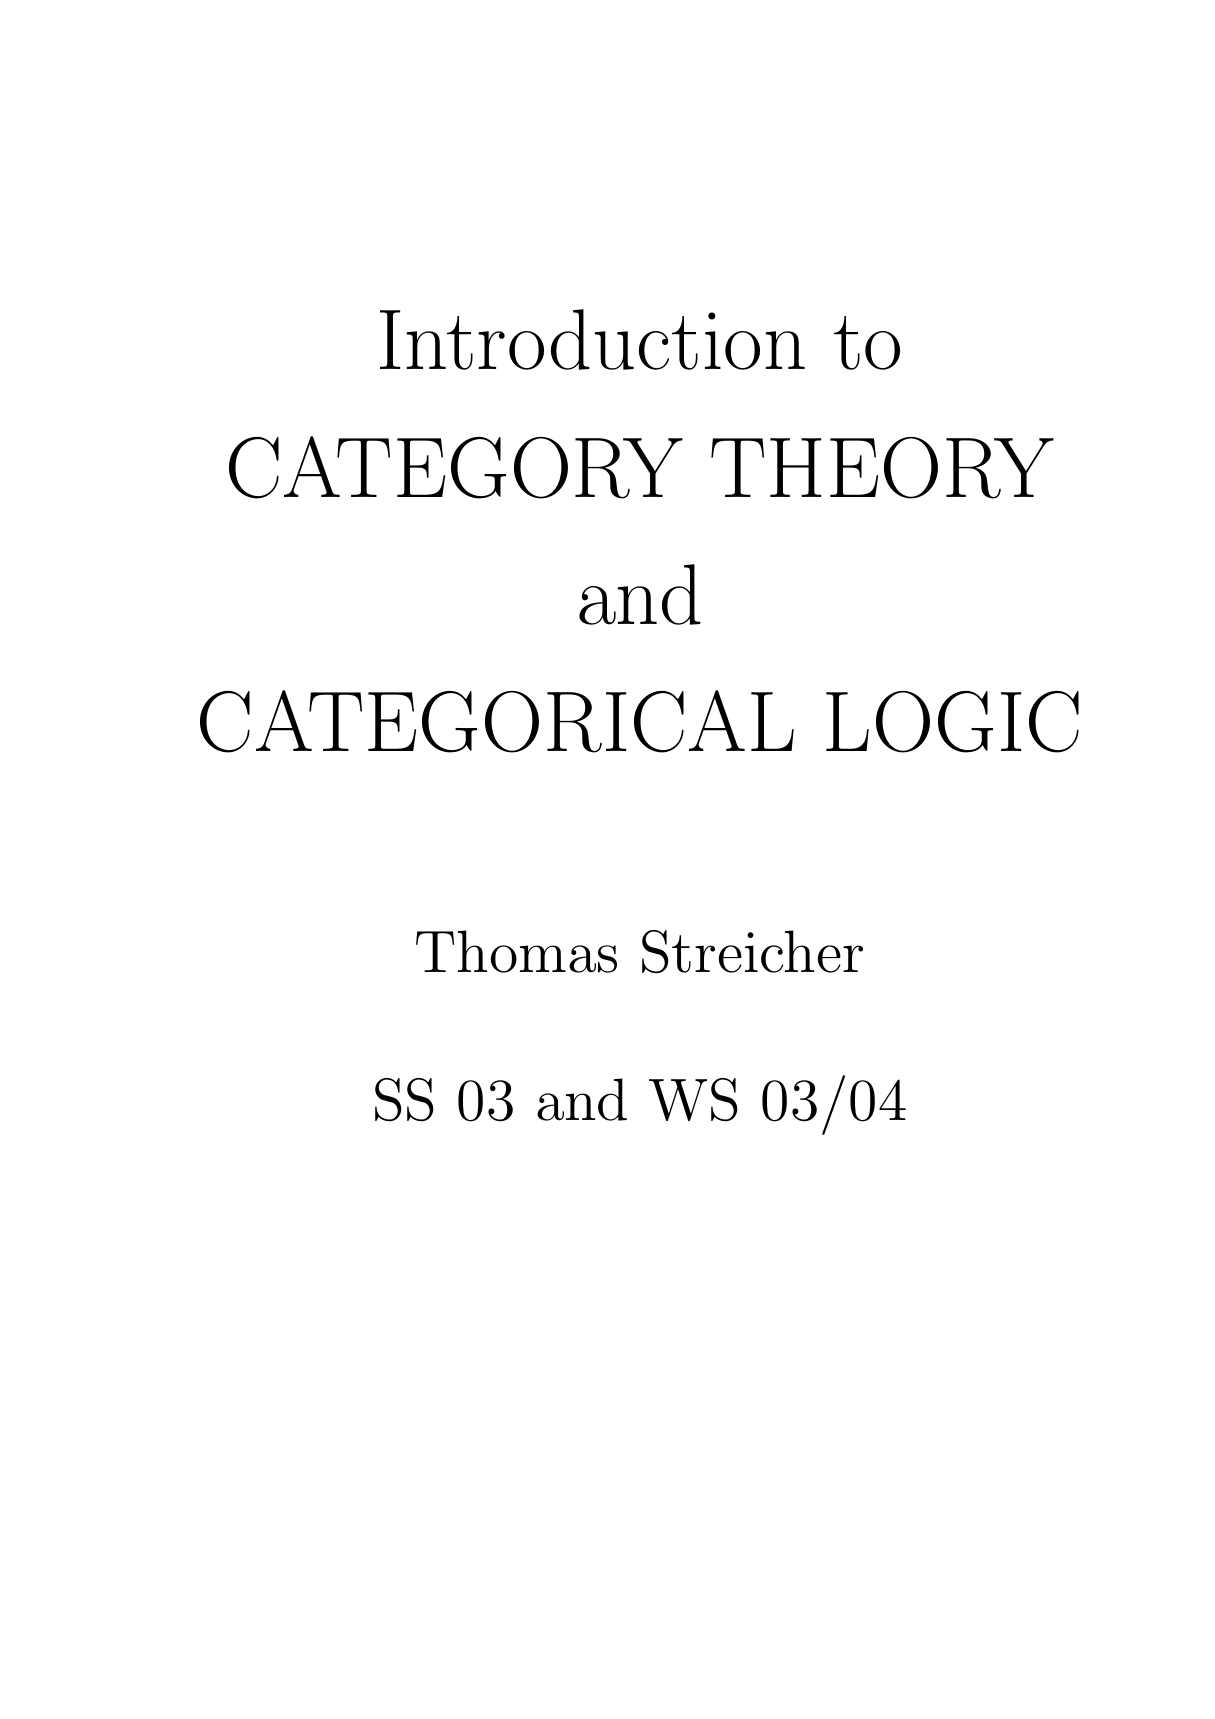
\includegraphics[height=3.5cm]{streicher-ctcl}}
  \end{center}

  We use an extension of the original form of the internal language which
  allows for unbounded quantification, Mike Shulman's
  \fixedhref{https://arxiv.org/abs/1004.3802}{\emph{stack semantics}}.
  (Independently, Steve Awodey, Carsten Butz, Alex Simpson and Thomas Streicher
  developed a
  \fixedhref{http://homepages.inf.ed.ac.uk/als/Research/Sources/set-models.pdf}{similar
  semantics}.)}
\end{frame}

% DURING THE TALK: Mention Set as a special case
% DURING THE TALK: Mention Mike and Awodey, Butz, Simpson, Streicher


\section{Internalizing higher direct images}

\begin{frame}{Internalizing higher direct images}
  \begin{block}{}
    A set~$M$ is \hil{injective} iff for any injection~$A \to B$,
    any map~$A \to M$ extends to a map on~$B$.
  \end{block}
  \vspace*{-1em}

  \begin{itemize}
    \small
    \item ``A set is injective iff it's inhabited'' is
          a \hil{constructive taboo}.
    \item Constructively, there are still \hil{enough injective sets}.
          % Every set~$M$ embeds into an injective set, for instance~$P(M)$ or~$P_{\leq1}(M)$.
    \item Any injective set is flabby.
  \end{itemize}
  \pause

  \begin{block}{}
    A module~$M$ is \hil{injective} iff for any linear injection~$A \to B$,
    any linear map~$A \to M$ extends to a linear map on~$B$.
  \end{block}
  \vspace*{-1em}

  \begin{itemize}
    \small
    \item It's consistent with \textbf{ZF} that there are no injective modules
    \href{https://www.ams.org/journals/tran/1979-255-00/S0002-9947-1979-0542870-6/S0002-9947-1979-0542870-6.pdf}{[Blass 1979]}.
    \item The existence of enough injective modules is \hil{constructively neutral}.
  \end{itemize}
  \pause

  \begin{block}{}
    \justifying
    A sheaf of modules~$M$ is \hil{injective} iff for any linear monomorphism
    \mbox{$A \!\!\to\!\! B$,
    any linear morphism~$A \!\!\to\!\! M$ extends to a linear morphism on~$B$.}
  \end{block}
  \vspace*{-1em}

  \begin{itemize}
    \small
    \item Assuming choice, there are enough injectives over any site.
    \item Assuming Zorn's lemma, a sheaf of modules over a locale~$X$ is injective iff, from the internal
    point of view of~$\Sh(X)$, it is an injective module.
  \end{itemize}

  \jnote{2-3}{Somewhat surprisingly, even though the standard proof that there
  are enough injective modules requires the axiom of choice and even though
  it's consistent with Zermelo--Fraenkel set theory that the zero module is the
  only injective~$\ZZ$-module, the existence of enough injective modules is
  \emph{constructively neutral}, that is, does not imply a fundamentally
  nonconstructive principle like the law of excluded middle.

  Indeed, assuming the axiom of choice in the metatheory, the statement~``any
  module can be embedded into an injective module'' holds in the internal
  language of any Grothendieck topos. This is because, assuming the axiom of
  choice in the metatheory, any sheaf of modules over a site can be embedded
  into an injective sheaf of modules and, somewhat
  surprisingly, \ldots}

  \jnote{3}{\ldots{} a sheaf of modules is injective if and only if it is an
  injective module from the internal point of view. The~``$\Rightarrow$''
  direction is straightforward; the~``$\Leftarrow$'' direction is nontrivial:
  The external meaning of the internal existential quantifier is \emph{local}
  existence. Hence linear morphisms into a sheaf of modules which is injective from the internal
  point of view can \emph{locally} be extended. But
  these extensions need not be compatible, hence might not glue to a global
  extension. For the case of sheaves of abelian groups, this result is due to
  Roswitha Harting in an
  \fixedhref{https://www.tandfonline.com/doi/pdf/10.1080/00927878308822853}{1983
  paper of her}. The case of sheaves of modules is arguably also due to her,
  even though she states that the result doesn't hold for sheaves of modules.
  (Technology has improved since then, and using flabbiness as an organizing
  principle one can give a reasonably straightforward proof of the general
  statement.)

  In contrast, internally and externally projective modules do not coincide at
  all.}

  \jnote{4}{A consequence of the fact that internal and external injectivity
  coincides for sheaves of modules over locales is that we can interpret the
  higher direct images~$R^n f_*(Y, E)$ of a sheaf~$E$ of modules over an
  over-locale~$f : Y \to X$ as sheaf cohomology~$H^n(I(Y), E)$, where~$I(Y)$ is
  the internal locale of~$\Sh(X)$ corresponding to~$Y$.

  A basic application is the following. Any student in algebraic geometry
  needs, at some point in her life, to compute the cohomology of projective space.
  At a later point she needs to compute higher direct images
  along~$\mathbb{P}^n_S \to S$, where~$\mathbb{P}^n_S$ is a relative version of
  projective space. Since higher direct images are just internal
  sheaf cohomology, she can in fact skip the second computation.

  Further progress along these lines is hindered by the fact that we don't yet
  have a constructive account of sheaf cohomology.}
\end{frame}

% DURING THE TALK: Harting


\section{Flabby objects}

\begin{frame}{Flabby resolutions}
  \begin{block}{}
    A sheaf~$E$ on a space~$X$ is \hil{flabby} iff any local section~$s \in
    E(U)$ on an open~$U$ extends to a global section~$\bar s \in E(X)$: $\bar s|_U = s$.
  \end{block}
  \vspace*{-1em}

  \begin{itemize}
    \justifying
    %\item Injective sheaves of sets and injectives sheaves of modules are flabby.
    \item Assuming Zorn's lemma:

          A sheaf is flabby iff, from the internal point of view, it's a flabby
          set. \\[0.6em]
    \item Assuming the law of excluded middle:

          Any sheaf of modules over a topological space embeds into a flabby
          sheaf of modules. \\[0.6em]
    \item Assuming Zorn's lemma, flabby sheaves of modules are \hil{acyclic for the global sections functor}.
    Hence, assuming \bad{??}, sheaf cohomology and higher direct images can be computed using \hil{flabby resolutions}.
  \end{itemize}

  \jnote{1-}{Since we cannot show the existence of enough injective sheaves of
  modules (or even just plain modules) constructively, the definition of sheaf
  cohomology using injective resolutions doesn't work in a constructive
  setting. Classically it's known that \emph{flabby resolutions} can also be
  used to compute sheaf cohomology. There are more flabby sheaves than injective
  ones, they have better stability properties (flabby sheaves are preserved
  under pushforward) and the axiom of choice is not needed to construct flabby
  resolutions (the standard proof uses only the law of excluded middle, and not
  Zorn's lemma). Hence it seems reasonable to base a constructively sensible
  definition of sheaf cohomology on flabby resolutions. We tried to do so, and
  failed.

  Assuming Zorn's lemma, the notion of a flabby sheaf is a local notion,
  meaning that a sheaf is flabby if and only if its restrictions to every
  member of an open covering are, but this fact is not obvious from the
  definition. In contrast, the notion that a sheaf~$E$ is flabby from the
  internal point of view is local without any assumptions (as is any
  internal notion), hence maybe we should consider adopting internal flabbiness as the
  official definition of flabbiness. Its external translation is:

  A sheaf~$E$ is flabby from the internal point of view if and only if for any
  local section~$s \in E(U)$, there is an open covering~$X = \bigcup_i U_i$
  such that for all~$i$, the section~$s$ extends to a section on~$U \cup U_i$.}
\end{frame}

\begin{frame}{Flabbiness as an organizing principle}
  \justifying\small
  \textbf{Proposition.} Let~$M$ be a sheaf of modules over a locale~$X$.
  Then~$M$ is injective iff it is injective from the point of view of~$\Sh(X)$.

  \textbf{Proof.} (Only ``$\Leftarrow$''.) Let~$i : A \to B$ be a linear
  monomorphism. Let~$f : A \to M$ be a linear morphism. We verify, internally, that
  the set~$E \defeq \{ \bar f : B \to M \,|\, \bar f \circ i = f \}$ is flabby.
  \pause

  Let~$K \subseteq E$ be a subterminal.
  We consider the injectivity diagram
  \[ \xymatrix{
    i[A] + B' \ar@{^{(}->}[r]\ar[d]_g & B \ar@{-->}@/^/[ld]^{\bar g} \\
    I
  } \]
  where~$B' \defeq \{ t \in B \,|\, \text{$t = 0$ or $K$ is
  inhabited} \} \subseteq B$ and~$g$ is defined as follows:
  Let~$s \in i[A] + B'$. Then~$s = i(a) + t$ for some~$a \in A$ and~$t \in B'$.
  Since~$t \in B'$, $t = 0$ or~$K$ is inhabited. If~$t = 0$,
  we set~$g(s) \defeq f(a)$. If~$K$ is inhabited, we set~$g(s) \defeq f(a) +
  \bar{f}(s)$, where~$\bar{f}$ is any element of~$K$.

  Since~$M$ is injective, there exists a dotted map~$\bar g \in E$.
  We have~$K \subseteq \{ \bar g \}$. \qed

  \jnote{1-}{The notion of being flabby from the internal point of view turns
  out to have valuable organizing power. For instance, both of the
  following statements can be proven by first verifying that a certain sheaf is
  internally flabby (which can be done entirely constructively) and then
  appealing to Zorn's lemma in order to obtain a global section of that sheaf.

  \begin{itemize}\justifying
    \item Flabby sheaves are acyclic for the global sections functor: Let~$0
    \to E \to F \to G \to 0$ be a short exact sequence of sheaves of modules
    and let~$E$ be flabby. Then the sequence remains exact after taking global
    sections.

    (Verify that the sheaf of local preimages of a given section~$s \in G(X)$ is
    flabby.)

    \item Internally injective modules are externally injective.

    (See proof on the slide.)
  \end{itemize}}
\end{frame}


\section[In the ef{}fective topos]{Flabbiness in the ef{}fective topos}

\begin{frame}{Flabbiness in the ef{}fective topos}
  \small
  \begin{block}{}
    A set~$M$ is \hil{flabby} iff any \pointthisbelow{<1>}{subterminal}{$\forall x,y
    \in K\_ x = y$}~$K \subseteq M$ is a \pointthisbelow{<1>}{subsingleton}{$\exists
    a \in M\_ K \subseteq \{a\}$}.
  \end{block}
  \bigskip
  \bigskip
  \bigskip

  \justifying
  \textbf{Proposition.}
  Let~$X$ be an ef{}fective object in the ef{}fective topos. Then
  \[ \text{``If~$X$ is flabby, any endomap on~$X$ has a fixed point.''} \]
  from the point of view of the ef{}fective topos.

  \textbf{Proof (sketch).}
  We have a procedure which computes for any subterminal~$K \subseteq X$ an
  element~$a_K$ such that~$K \subseteq \{ a_K \}$. Let~$f : X \to X$ be a map.
  Construct~$K \defeq \{ f(a_K) \}$. Then~$K \subseteq \{ a_K \}$, so~$f(a_K) =
  a_K$. \qed
  \medskip

  \textbf{Corollary.}
  The only ef{}fective flabby module~$M$ is the zero module.

  \textbf{Proof.} Let~$x \in M$.
  Then~$x + a = a$ for some~$a \in M$; hence~$x = 0$. \qed

  \textbf{Proposition.}
  Assuming the law of excluded middle, any~$\neg\neg$-separated
  module in the ef{}fective topos can be embedded into a flabby module.

  \textbf{Proof.} We have~$M \hookrightarrow \Delta\Gamma M$. \qed
  \medskip

  \textbf{Question.} Are there enough flabby modules in the ef{}fective topos?

  \jnote{1-}{The notion of flabby sets was conceived to model the notion of
  flabby sheaves and is therefore closely connected to Grothendieck toposes.
  Hence it is instructive to study flabby objects in elementary toposes which
  are not Grothendieck toposes, away from their original conceptual home.

  In particular, we hope to prove the conjecture that the statement ``any
  module embeds into a flabby module'' is not constructively provable by
  verifying that it doesn't hold in the ef{}fective topos.

  To this end, the slide displays two results.

  Details on the self-referential construction~``$K \defeq \{ f(a_K) \}$'' are in
  \fixedhref{https://rawgit.com/iblech/internal-methods/master/paper-flabby-objects.pdf}{this
  draft paper}. A module is~$\neg\neg$-separated if and only if~$\neg\neg(x = 0)$ implies~$x = 0$.
  References on the ef{}fective topos include Martin Hyland's
  \fixedhref{https://webdpmms.maths.cam.ac.uk/~martin/Research/Oldpapers/hyland-effectivetopos.pdf}{survey
  paper} and the canonical book by one of our honoraries:

  {\centering\fixedhref{https://www.staff.science.uu.nl/~ooste110/boekbegin.pdf}{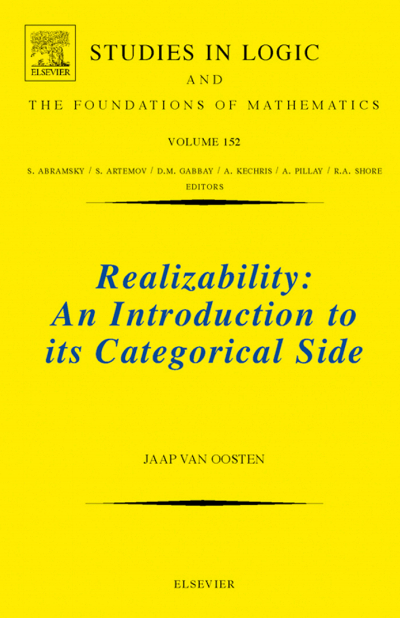
\includegraphics[height=3.5cm]{oosten-realizability}}\par}}
\end{frame}

\begin{frame}{State of affairs}
  \centering

  \textcolor{blue!90}{\Huge \smiley}

  The existence of enough injective modules is constructively neutral. \\
  Higher direct images can be understood as internal sheaf cohomology.

  \bigskip

  \bad{\Huge \scalebox{2}{\frownie}}

  Flabby sheaves can fail to be acyclic, constructively. \\
  There is still no general constructive framework for sheaf cohomology. \\
  Even though:

  \begin{itemize}
    \item Basic homological algebra is entirely constructive.
    \item There are algorithms for computing cohomology [Barakat, \ldots].
    \item Čech methods work constructively, even in a synthetic context.
  \end{itemize}

  \jnote{1-}{Even if we could constructively prove that there are enough flabby
  modules, there is still the problem that the proof that flabby
  sheaves of modules are acyclic for the global sections functor (appears to)
  require Zorn's lemma.

  Hence it appears that the simple idea of basing a constructive account of sheaf cohomology on flabby
  resolutions doesn't work.

  More work is needed.
  I hope that some day, we can study the cohomology of the smallest dense
  sublocale of the one-point space.$^\star$

  {\centering
\includegraphics[height=2cm]{phantoms}\par}

  $^\star$ Assuming the law of excluded middle, this locale is just
  the one-point space again. Hence cohomology of this locale should measure the
  extent to which we're nonclassical, being zero if and only if the law of
  excluded middle holds.

  An alternative way of putting this question is as follows.
  Let~$\Set_{\neg\neg}$ be the smallest dense subtopos of~$\Set$, the topos of
  double negation sheaves. The forgetful functor~$\mathrm{Ab}(\Set_{\neg\neg})
  \to \mathrm{Ab}$ is left-exact, but might not be right-exact, since
  a map~$f : A \to B$ is an epimorphism
  in~$\mathrm{Ab}(\Set_{\neg\neg})$ if and only if~$\forall y \in B\_
  \neg\neg(\exists x \in A\_ f(x) = y)$, which is weaker than being surjective.
  What do its right derived functors look like?\par}
\end{frame}
\addtocounter{framenumber}{-1}

\end{document}
